\documentclass{article}

\usepackage[final]{style}
\usepackage[utf8]{inputenc} % allow utf-8 input
\usepackage[T1]{fontenc}    % use 8-bit T1 fonts
\usepackage{hyperref}       % hyperlinks
\usepackage{url}            % simple URL typesetting
\usepackage{booktabs}       % professional-quality tables
\usepackage{amsfonts}       % blackboard math symbols
\usepackage{nicefrac}       % compact symbols for 1/2, etc.
\usepackage{microtype}      % microtypography
\usepackage{verbatim}
\usepackage{graphicx}       % for figures
\usepackage{subcaption}
\usepackage{float}


\title{Lecture 15: Detecting Objects by Parts}

\author{
  David R. Morales, Austin O. Narcomey, Minh-An Quinn, Guilherme Reis, Omar Solis \\
  Department of Computer Science\\
  Stanford University\\
  Stanford, CA 94305 \\
  \texttt{\{mrlsdvd, aon2, minhan, greis, osolis9\}@stanford.edu} 
}

\begin{document}

\maketitle


\section{Introduction to Object Detection}
Previously, we introduced methods for detecting objects in an image; in this lecture, we describe methods that detect and localize generic objects in images from various categories such as cars and people. The categories that are detected depend on the application domain. For example, self-driving cars need to detect other cars and traffic signs.
\begin{figure}[h]
	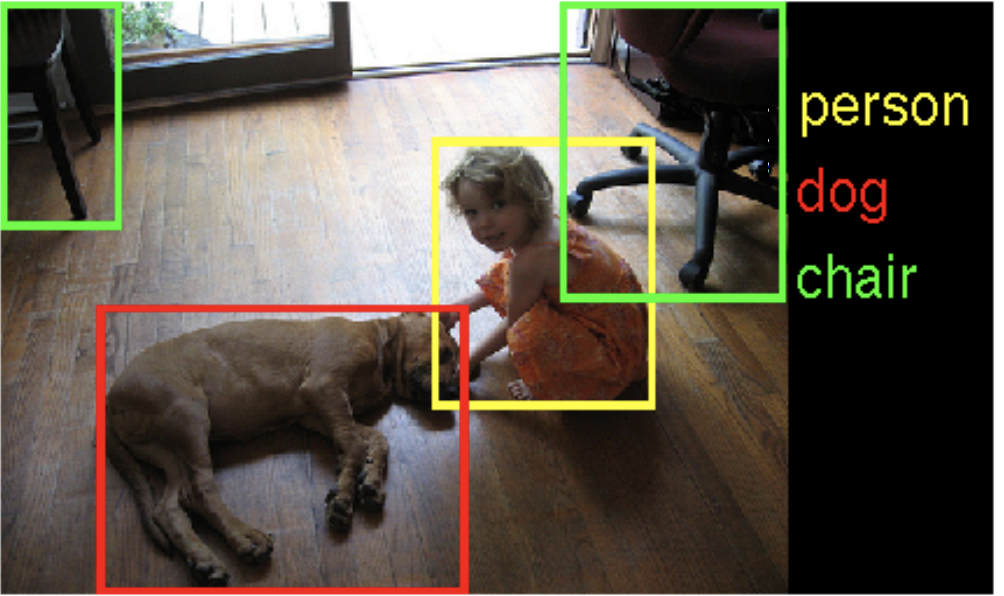
\includegraphics[width=\textwidth]{object-detector-intro.png}
    \caption{An example of an object detection algorithm detecting the categories of a person, dog, and a chair}
\end{figure}

\subsection{Challenges}
Object detection, however, faces many challenges. The challenges include the varying illumination conditions, changes in the viewpoints, object deformations, and intra-class variability; this makes objects of the same category appear different and makes it difficult to correctly detect and classify objects. In addition, the algorithms introduced herein only give the 2D location of the object in the image and not the 3D location. For example, the algorithms cannot determine if an object is in front or behind another object. Additionally, the following object detectors do not provide the boundary of an object it finds; the object detector just provides a bounding box of where the object was found.

\section{Current Object Detection Benchmarks}
Today, object detection has practically been addressed for certain applications such as face detection. To evaluate the performance of an object detector, researchers use standardized object detection benchmarks. Benchmarks are used to make sure we are moving forward and performing better with new research.

\subsection{PASCAL VOC} 
The first widely used benchmark was the PASCAL VOC Challenge \cite{pascal-voc-2012}, or the Pattern Analysis, Statistical Modeling, and Computational Learning Visual Object Classes challenge. The PASCAL VOC challenge was used from 2005 to 2012 and tested 20 categories. PASCAL was regarded as a high quality benchmark because its test categories had high variability within each category. Each test image also had bounding boxes for all objects of interest like cars, people, cats, etc. PASCAL also had annual classification, detection, and segmentation challenges.

\subsection{ImageNet Large Scale Visual Recognition Challenge}
The benchmark that replaced PASCAL is the ImageNet Large Scale Visual Recognition Challenge (ILSVR) \cite{ILSVRC15}. The ILSVR Challenge tested 200 categories of objects, significantly more than what PASCAL tested, had more variability in the object types, and had many objects in a single image.

\begin{figure}[h]
	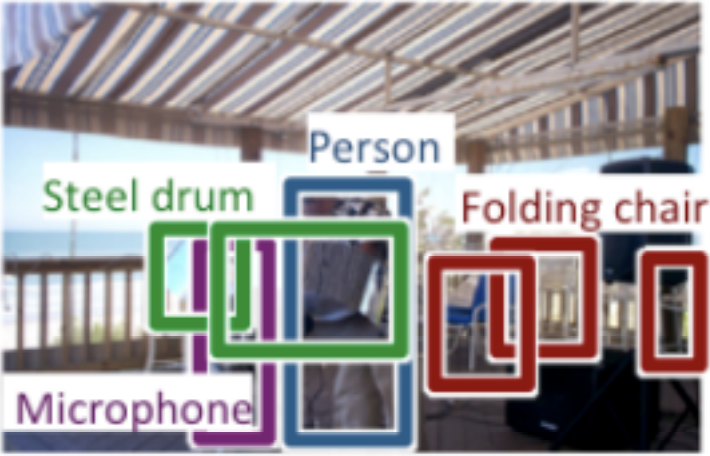
\includegraphics[width=\textwidth]{ilsvr.png}
    \caption{An example of a labeled ILSVR test image.}
\end{figure}

\subsection{Common Objects in Context}
Another benchmark that is still used today is the Common Objects in Context (COCO) challenge \cite{DBLP:journals/corr/LinMBHPRDZ14}. The COCO challenge tests 80 categories, but in addition to testing bounding boxes of locations of objects, it also tests object segmentation, which are detailed bounding areas of an object. Creating the test images for the dataset used in the COCO challenge is very time consuming because each object that is tested needs to be traced almost perfectly.

\begin{figure}[h]
	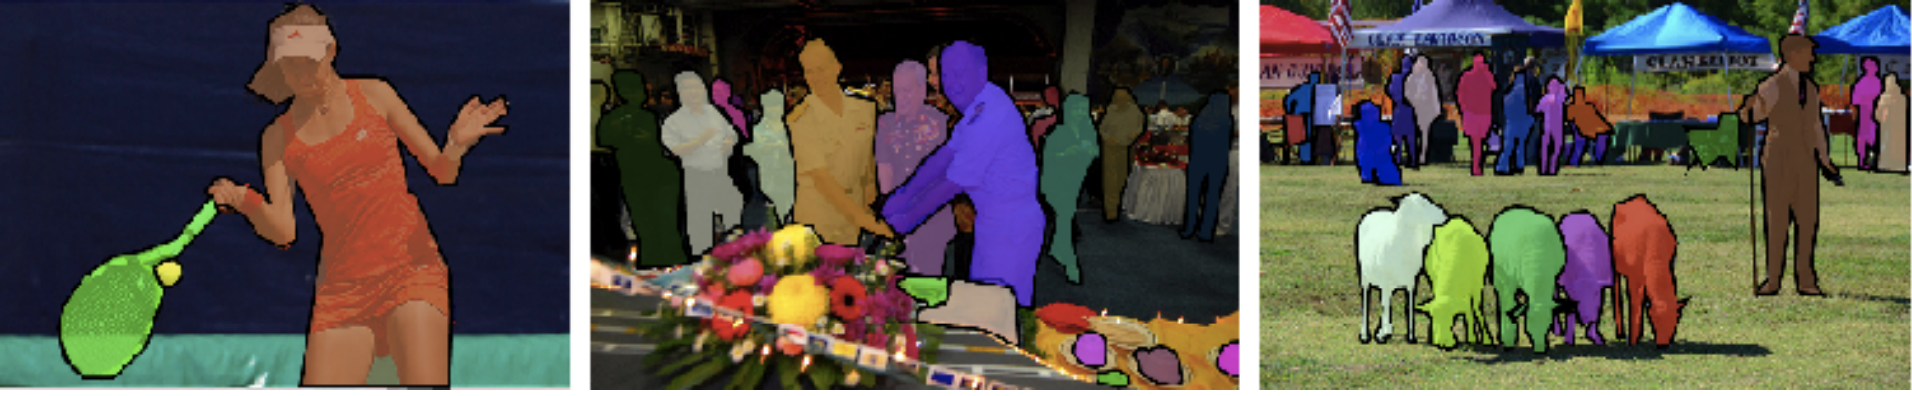
\includegraphics[width=\textwidth]{coco.png}
    \caption{Object segmentation used for the COCO challenge.}
\end{figure}

\pagebreak

\section{Evaluating Object Detection}

When evaluating an object detection algorithm, we want to compare the predictions with ground truth. The ground truth is provided by humans who manually classify and locate objects in the images.

\begin{figure}[ht]
\centering
	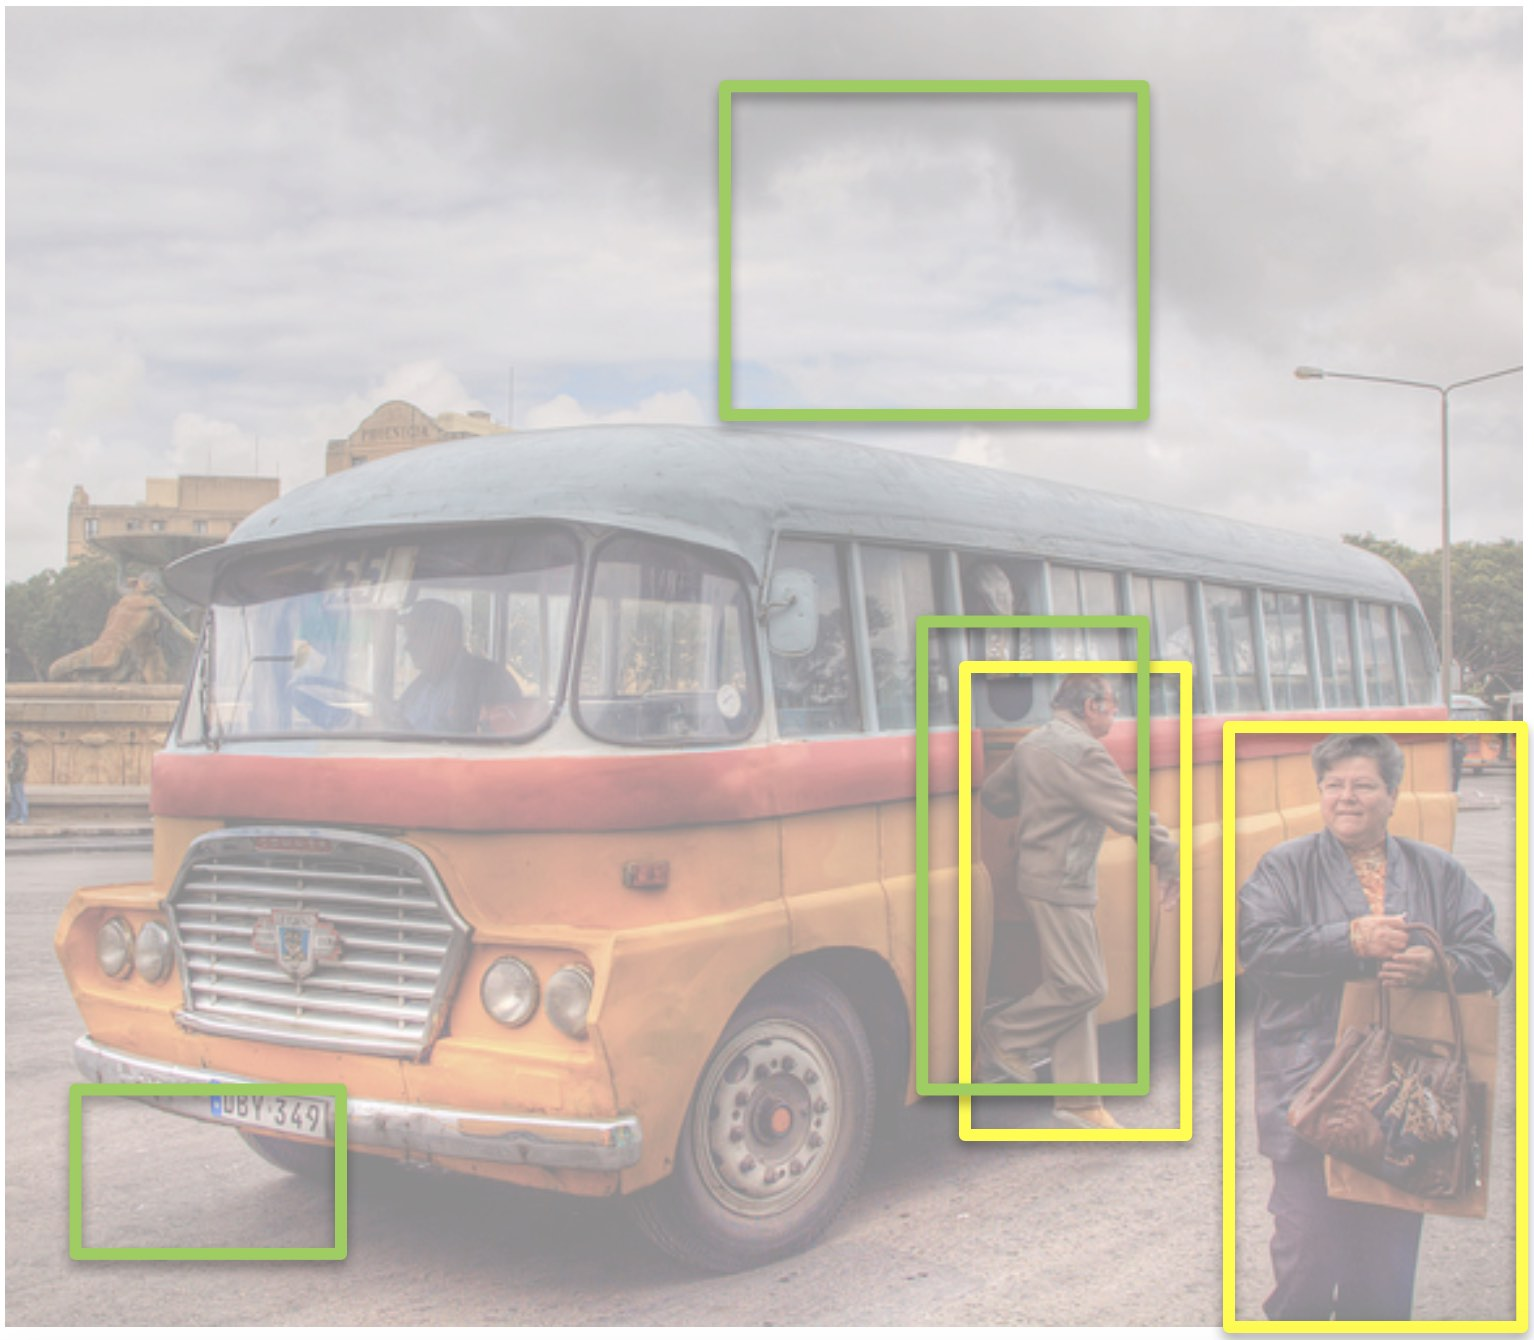
\includegraphics[width=0.8\textwidth]{predict_truth.jpg}
    \caption{Yellow boxes represent ground truth while green boxes are predictions.}
\end{figure}

When comparing predictions with ground truth, there are four different possibilities: \\

\textbf{1. \hspace{0.25cm} True Positive (TP)}\\
True positives are objects that both the algorithm (prediction) and annotator (ground truth) locate. In order to be more robust to slight variations between the prediction and ground truth, predictions are considered true positives when the overlap between the prediction and ground truth is greater than 0.5 (Figure \ref{fig:evaluations}a). The overlap between the prediction and ground truth is defined as the intersection over the union of the prediction and ground truth. True positives are also sometimes referred to as hits.\\

\textbf{2. \hspace{0.25cm} False Positive (FP)}\\
False positives are objects that the algorithm (prediction) locates but the annotator (ground truth) does not locate. More formally, false positives occur where the overlap of the prediction and ground truth is less than 0.5 (Figure \ref{fig:evaluations}b). False positives are also referred to as false alarms.\\

\textbf{3. \hspace{0.25cm} False Negative (FN)}\\
False negatives are ground truth objects that our model does not find (Figure \ref{fig:evaluations}b). These can also be referred to as misses.\\

\textbf{4. \hspace{0.25cm} True Negative (TN)}\\
True negatives are anywhere our algorithm didn’t produce a box and the annotator did not provide a box. True negatives are also called correct rejections.\\

\begin{figure}[h]
  \begin{subfigure}{0.32\textwidth}
    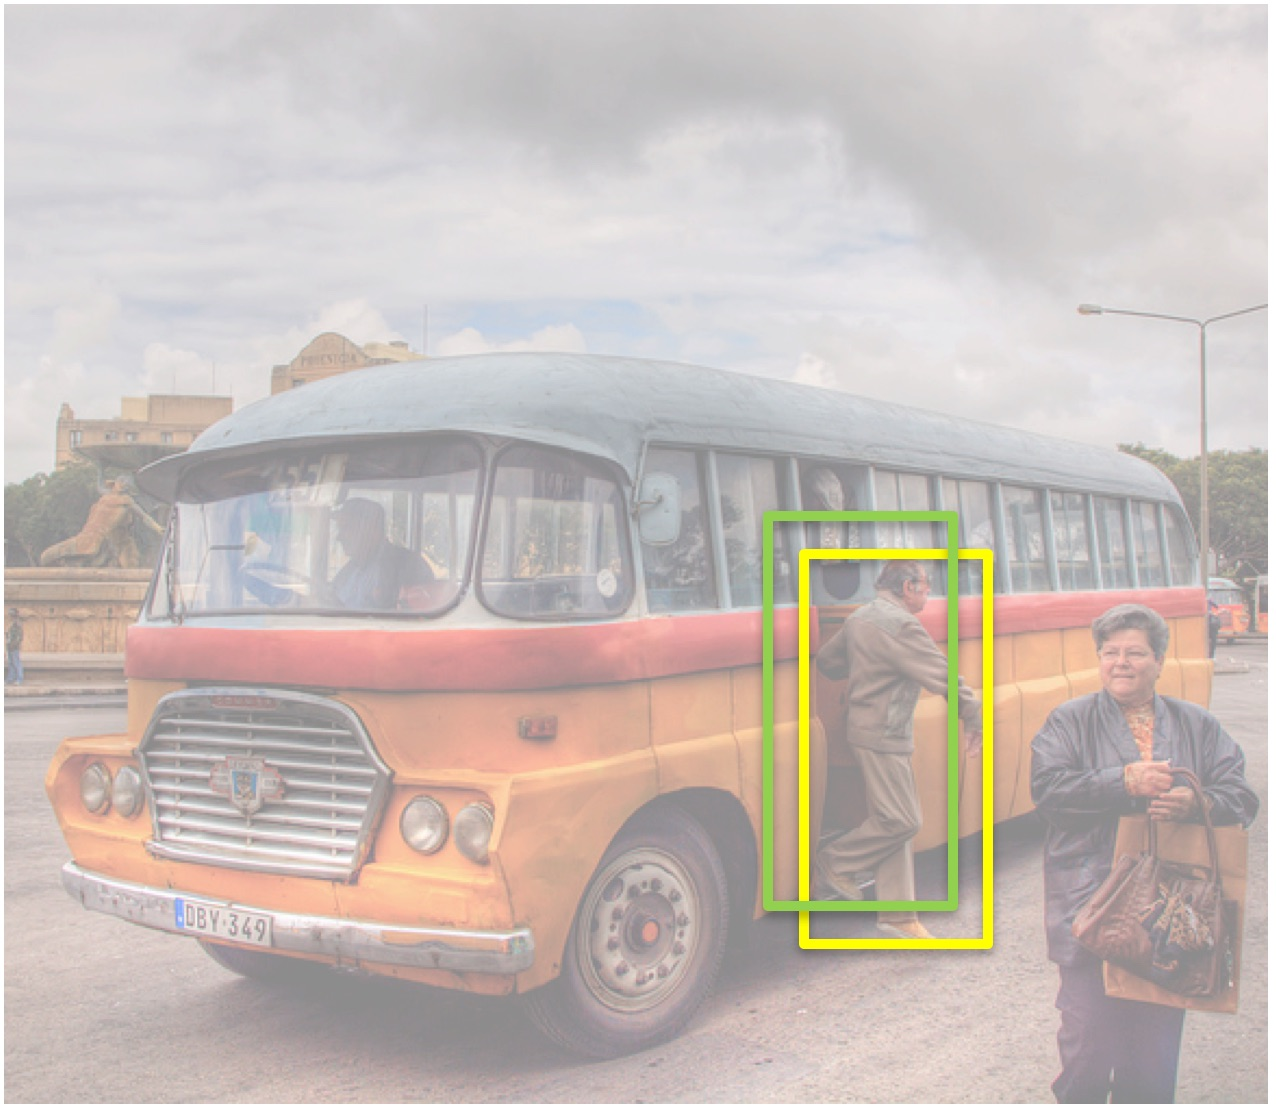
\includegraphics[width=\linewidth]{true_pos.jpg}
    \caption{}
  \end{subfigure}
  \hspace*{\fill} % separation between the subfigures
  \begin{subfigure}{0.32\textwidth}
    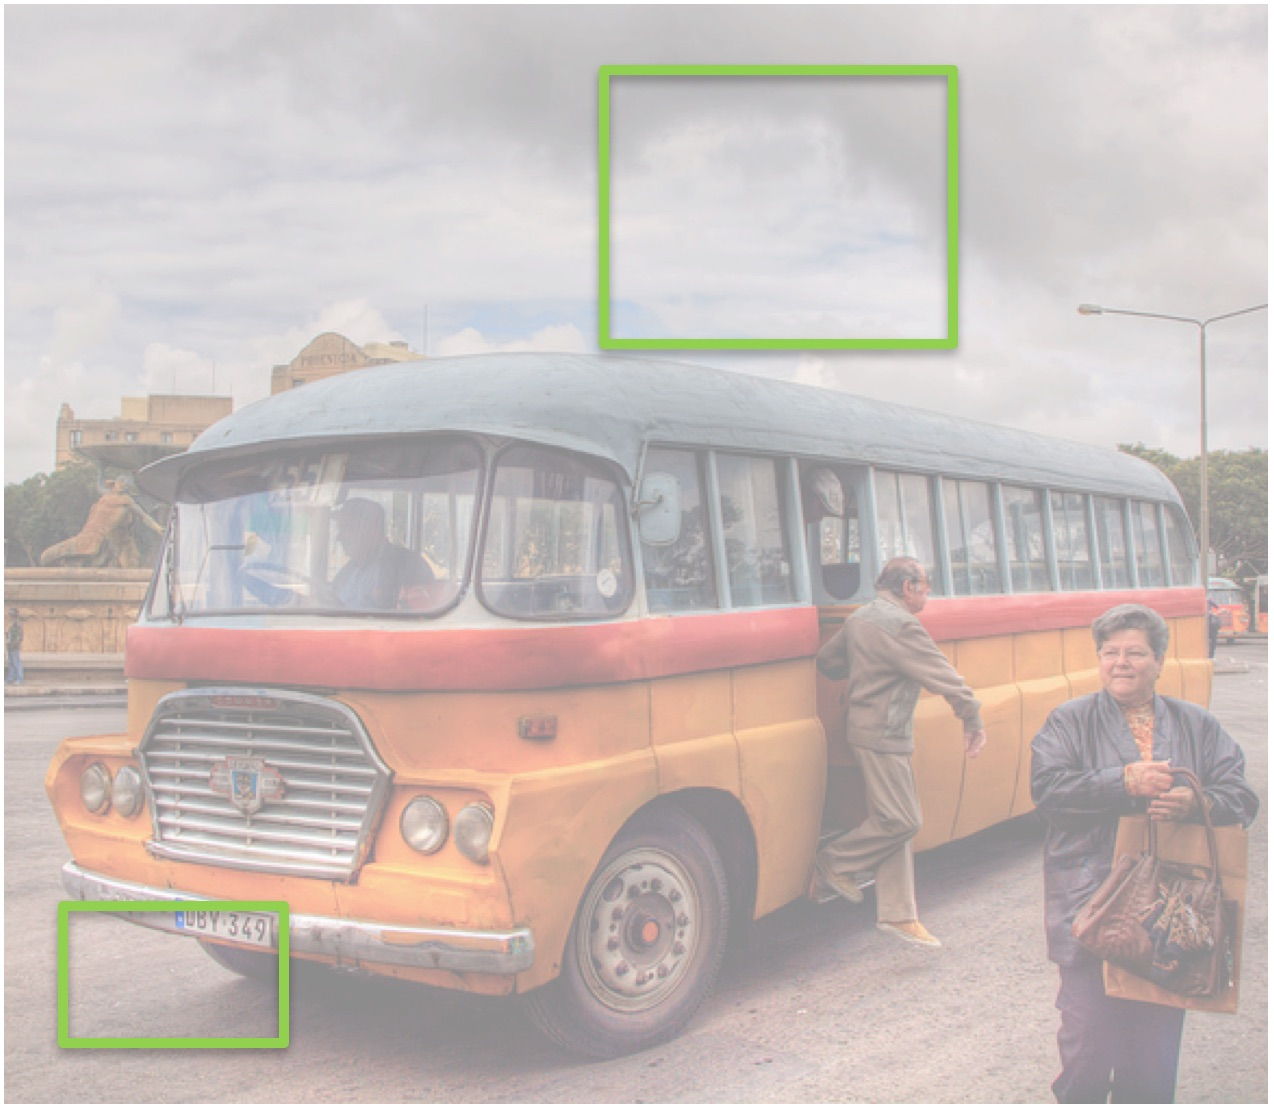
\includegraphics[width=\linewidth]{false_pos.jpg}
    \caption{}
  \end{subfigure}
  \hspace*{\fill} % separation between the subfigures
  \begin{subfigure}{0.32\textwidth}
    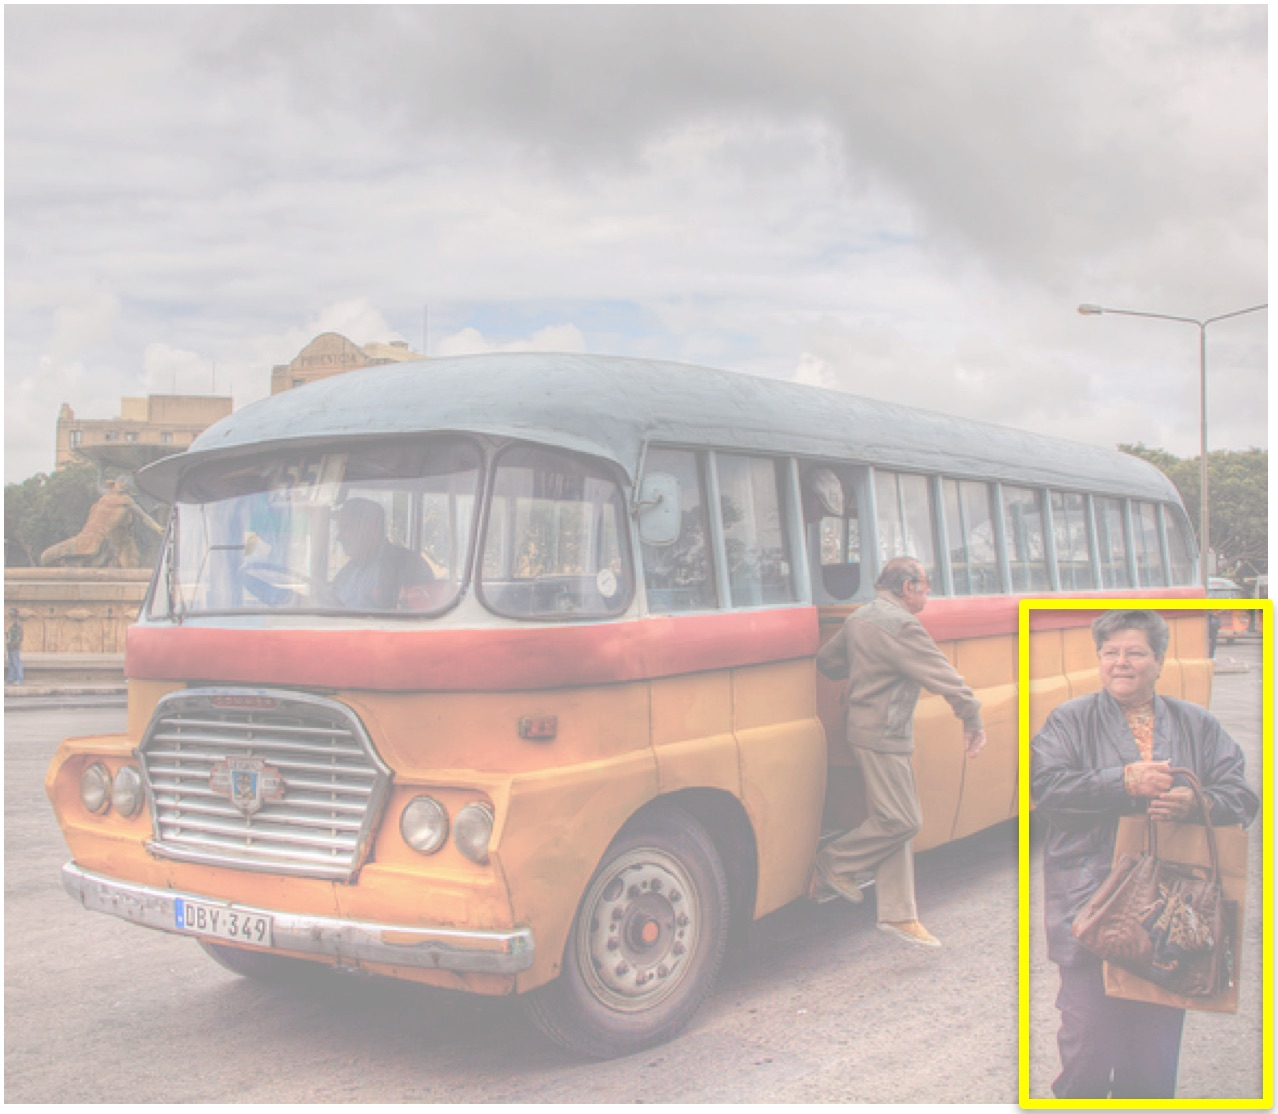
\includegraphics[width=\linewidth]{false_neg.jpg}
    \caption{}
  \end{subfigure}
  \hspace*{\fill} % separation between the subfigures
  \caption{Example classifications using an overlap threshold of 0.5. (a) True positive, because ground truth (yellow box) and prediction (green box) overlap is more than 0.5. (b) False positive, since the prediction boxes (green) do not overlap with any ground truth boxes. (c) False negative, since the ground truth box (yellow) is not detected by the model.}
  \label{fig:evaluations}
\end{figure}

\begin{figure}[ht]
\centering
	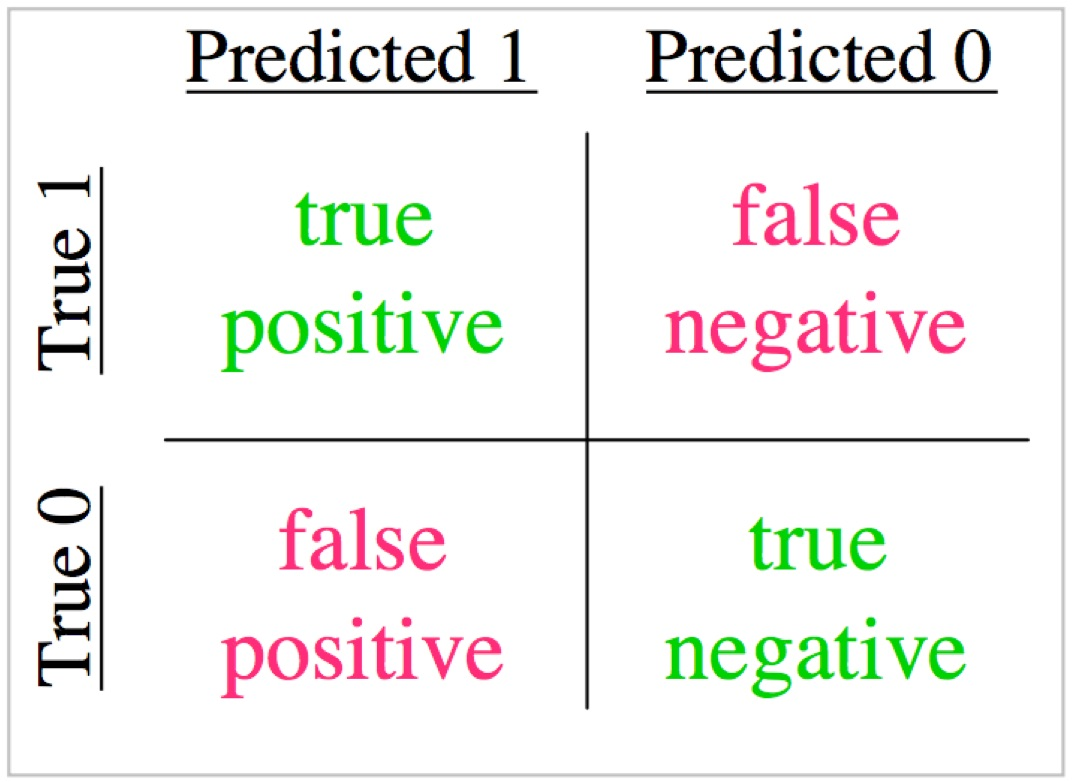
\includegraphics[width=0.8\textwidth]{chart.jpg}
    \caption{Summary chart of classifications, with green being counts you want to maximize and red being counts you want to minimize.}
    \label{fig:eval_chart}
\end{figure}


In general, we want to minimize false positives and false negatives while maximizing true positives and true negatives (Figure \ref{fig:eval_chart}.

Using the counts of true positives (TP), true negatives (TN), false positives (FP), and false negatives (FN), we can calculate two measures: precision and recall.

$$Precision = \frac{TP}{TP + FP}$$
Precision can be thought of as the fraction of correct object predictions among all objects detected by the model.

$$Recall = \frac{TP}{TP + FN}$$
Recall can be thought of as the fraction of ground truth objects that are correctly detected by the model. \\

\begin{figure}[ht]
\centering
	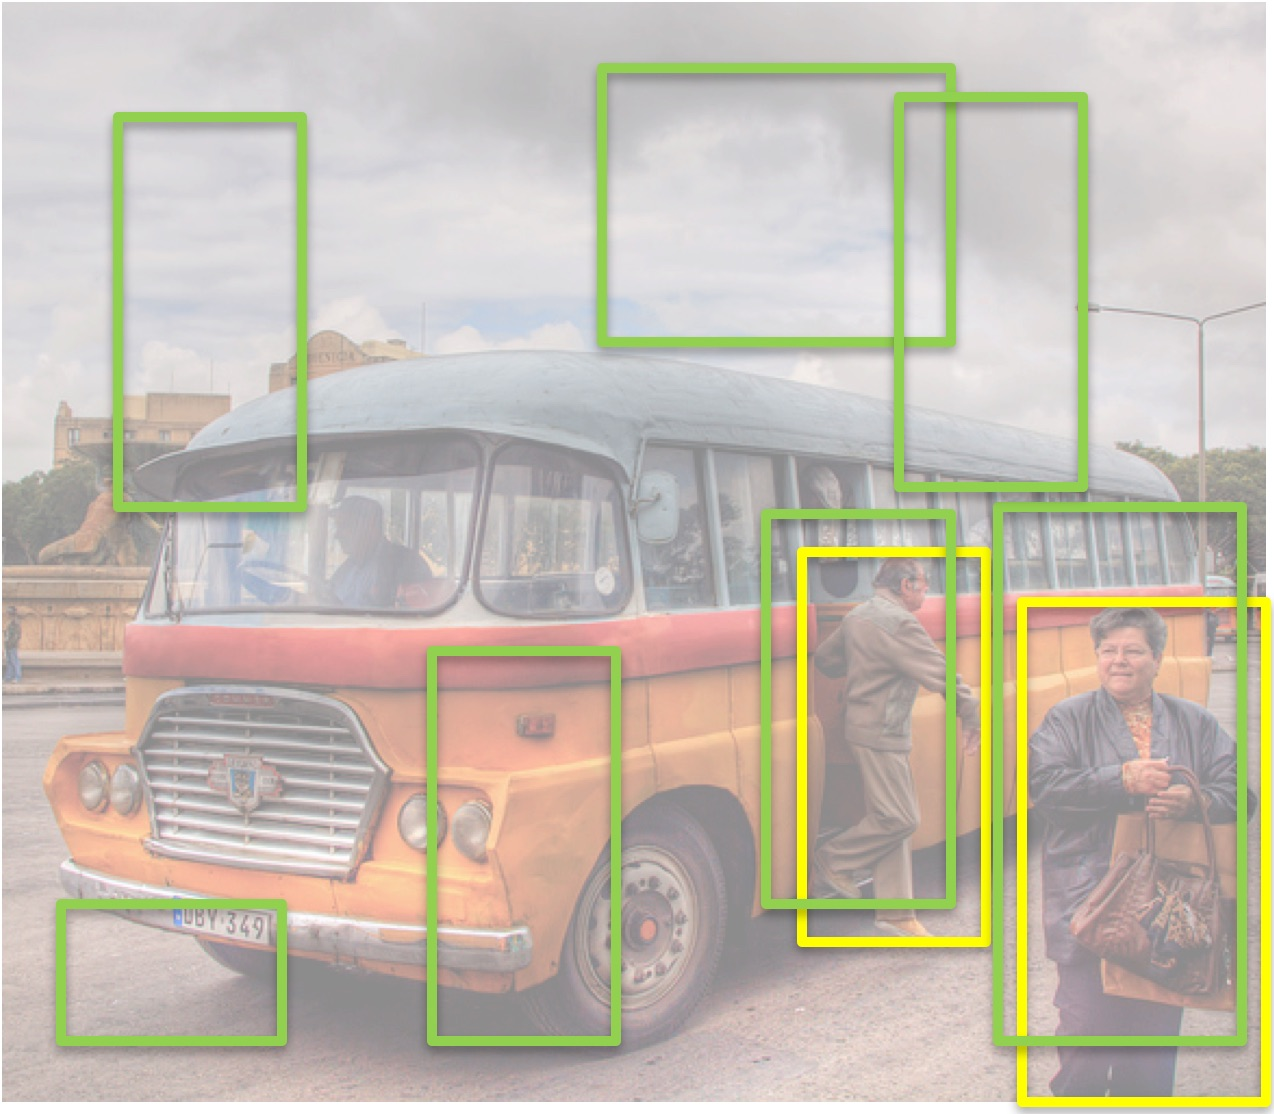
\includegraphics[width=0.8\textwidth]{prec_recall_pic.jpg}
    \caption{Predictions are green boxes while ground truth is yellow. All the ground truths are correctly predicted, making recall perfect. However, precision is low, since there are many false positives.}
\end{figure}

For every threshold we use to define true positives (In Figure \ref{fig:evaluations} the overlap threshold was set to 0.5), we can measure the precision and recall. Using that information, we can create a Precision-Recall curve (PR curve). Generally, we want to maximize both precision and recall. Therefore, for a perfect model, precision would be 1 and recall would be 1, for all thresholds. When comparing different models and parameters, we can compare the PR curves. The better models have more area under the curve. 

\begin{figure}[ht]
\centering
	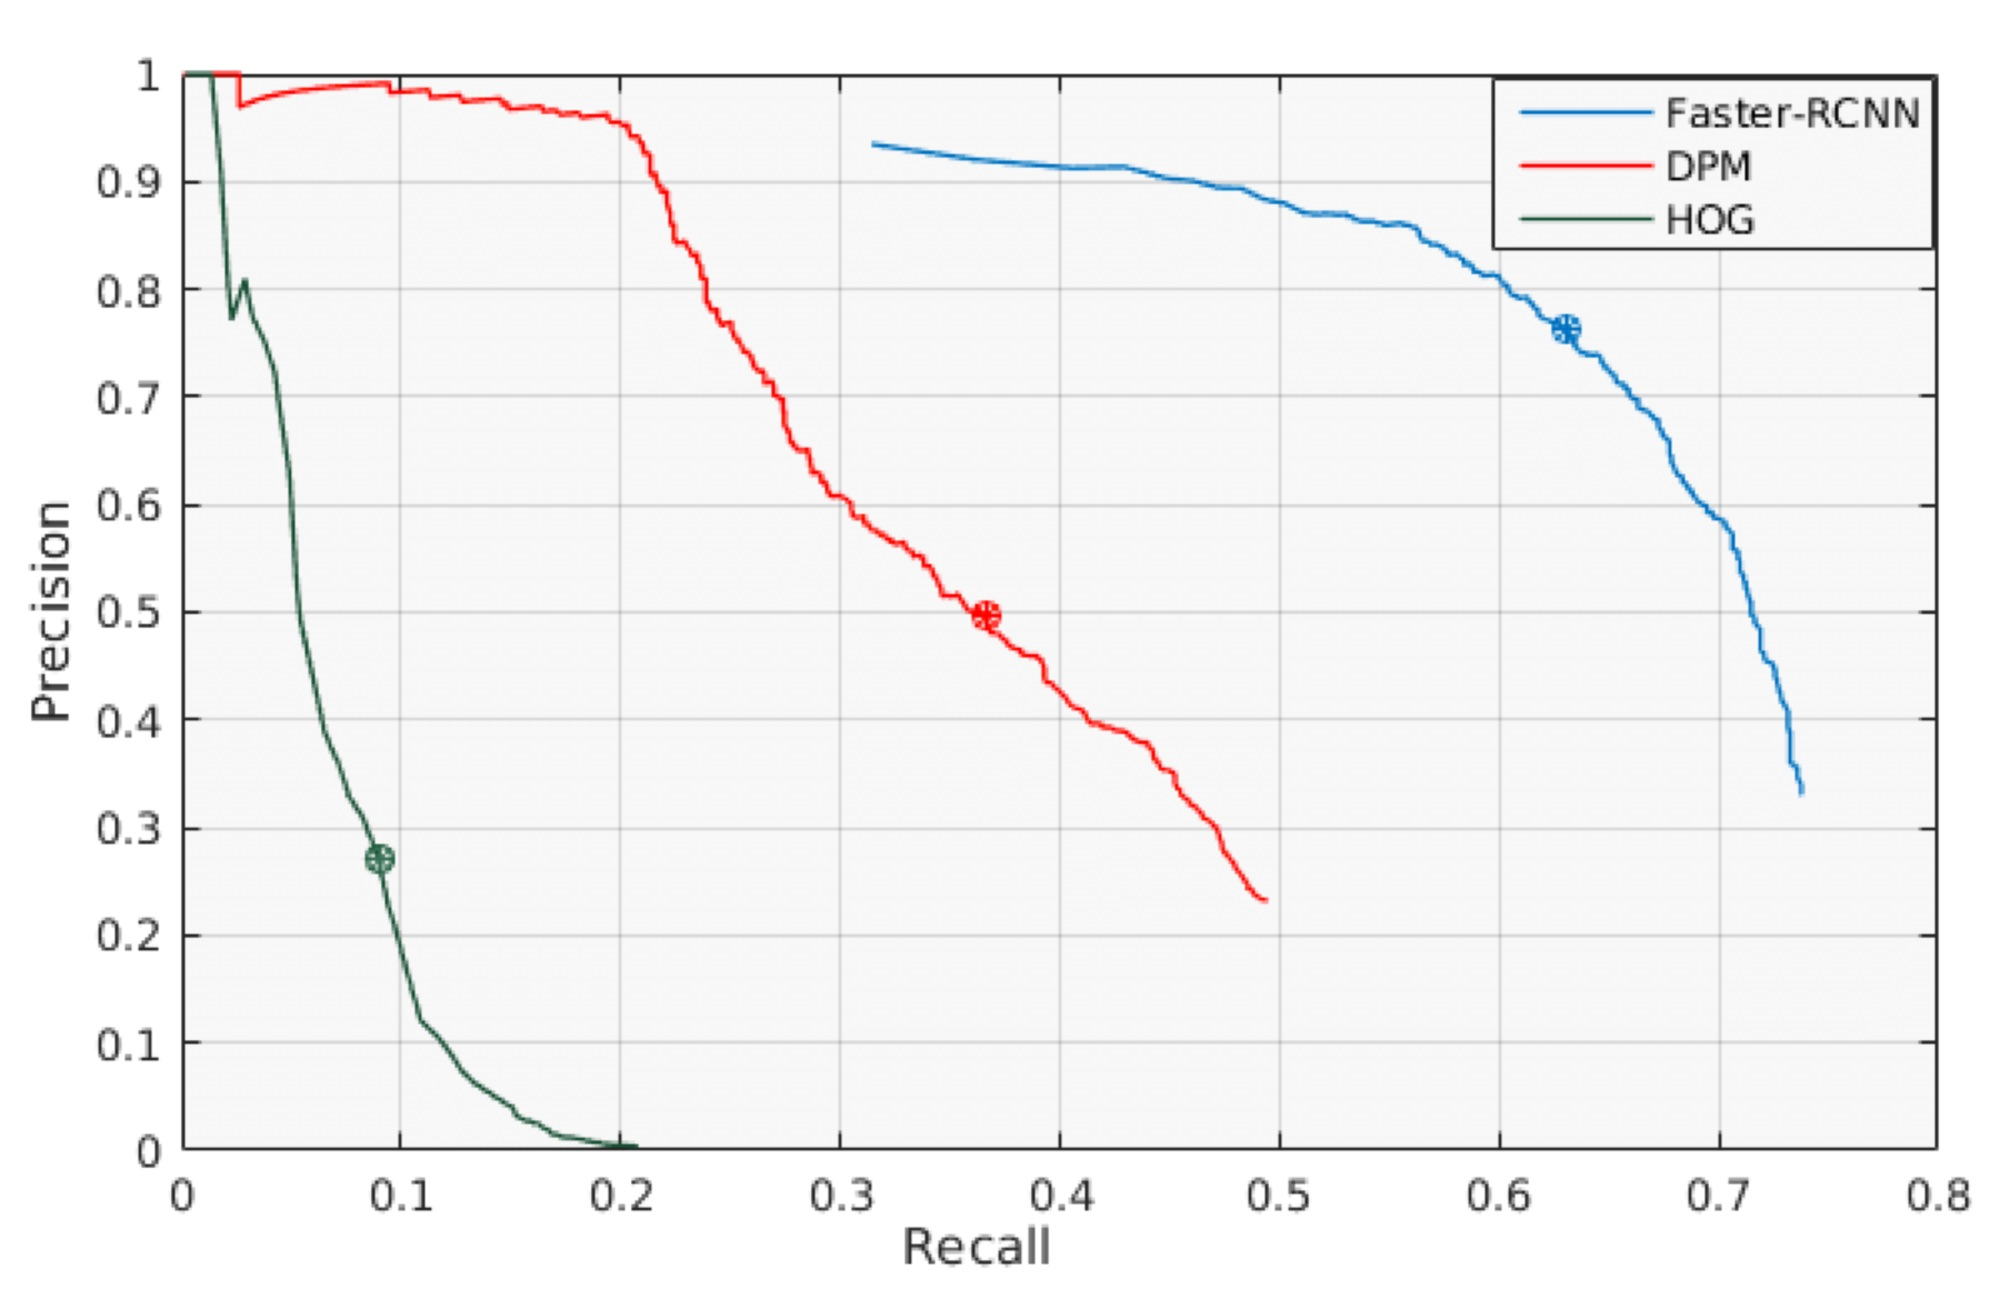
\includegraphics[width=0.8\textwidth]{precision_recall.jpg}
    \caption{Faster-RCNN model is the best of the three models since it has the most area under the curve.}
\end{figure}

However, depending on the application, we may want specific values for precision and recall. Therefore, you can choose the best model by fixing, say the recall, and finding the model that has the best precision at that recall.

We can also use the counts of TP, FP, TN, and FN to see how our model is making errors.


\section{A Simple Sliding Window Detector}
The detection can be treated as a classification problem. Instead of attempting to produce the location of objects in an image by processing the entire image at once, slide a window over the image and classify each position of the window as either containing an object or not (Figure \ref{fig:sliding_window}).

\begin{figure}[H]
  \begin{subfigure}{0.48\textwidth}
    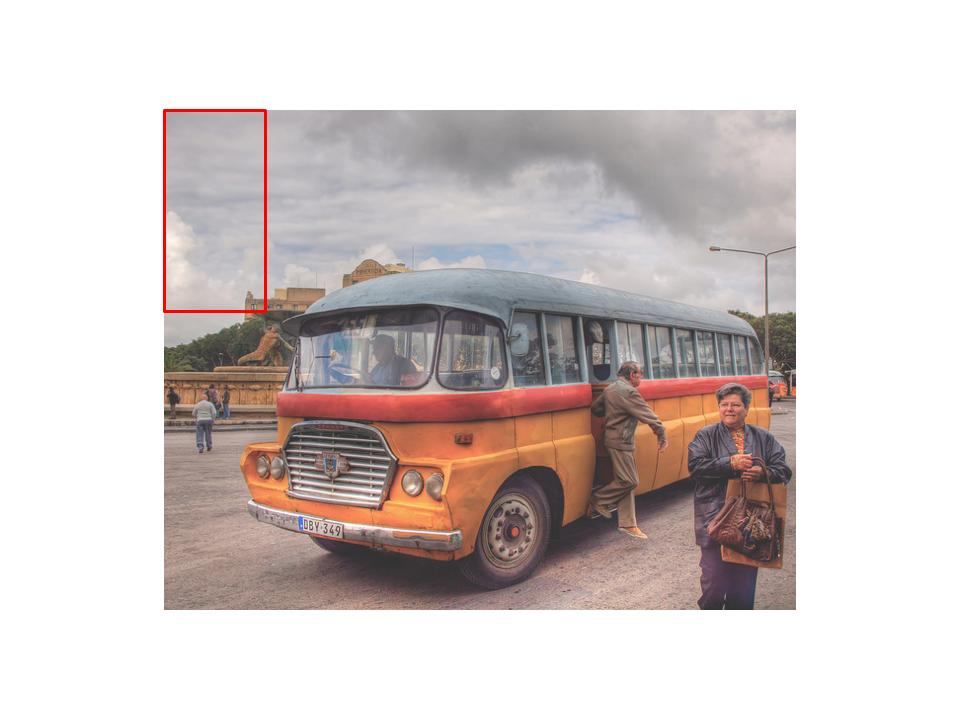
\includegraphics[width=\linewidth]{sliding_window_a.jpg}
    \caption{}
  \end{subfigure}
  \hspace*{\fill} % separation between the subfigures
  \begin{subfigure}{0.48\textwidth}
    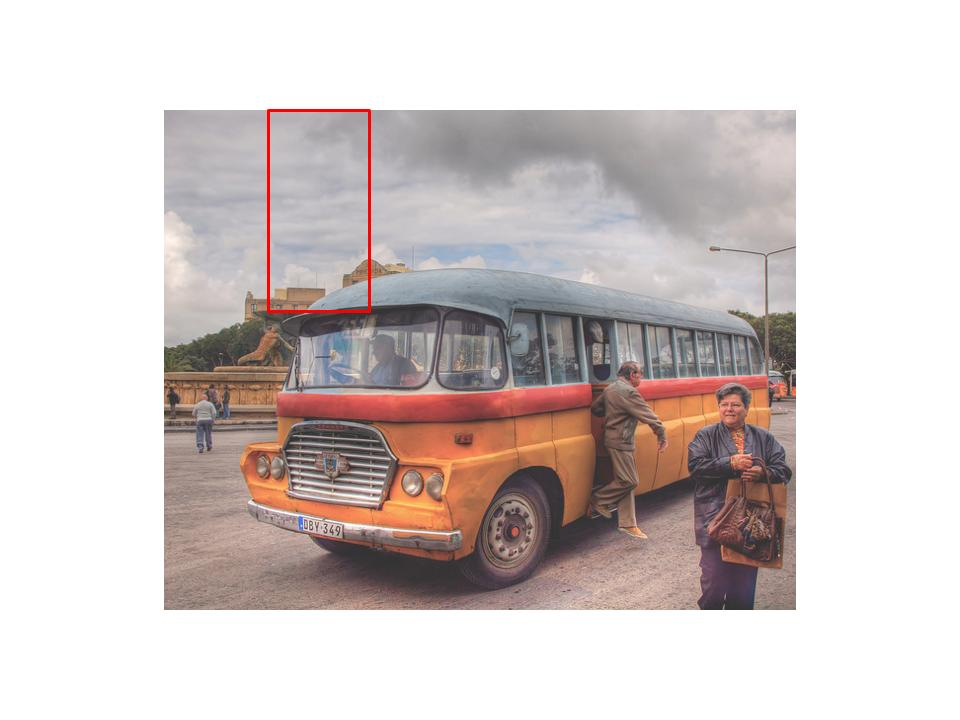
\includegraphics[width=\linewidth]{sliding_window_b.jpg}
    \caption{}
  \end{subfigure}
  \hspace*{\fill} % separation between the subfigures
  \begin{subfigure}{0.48\textwidth}
    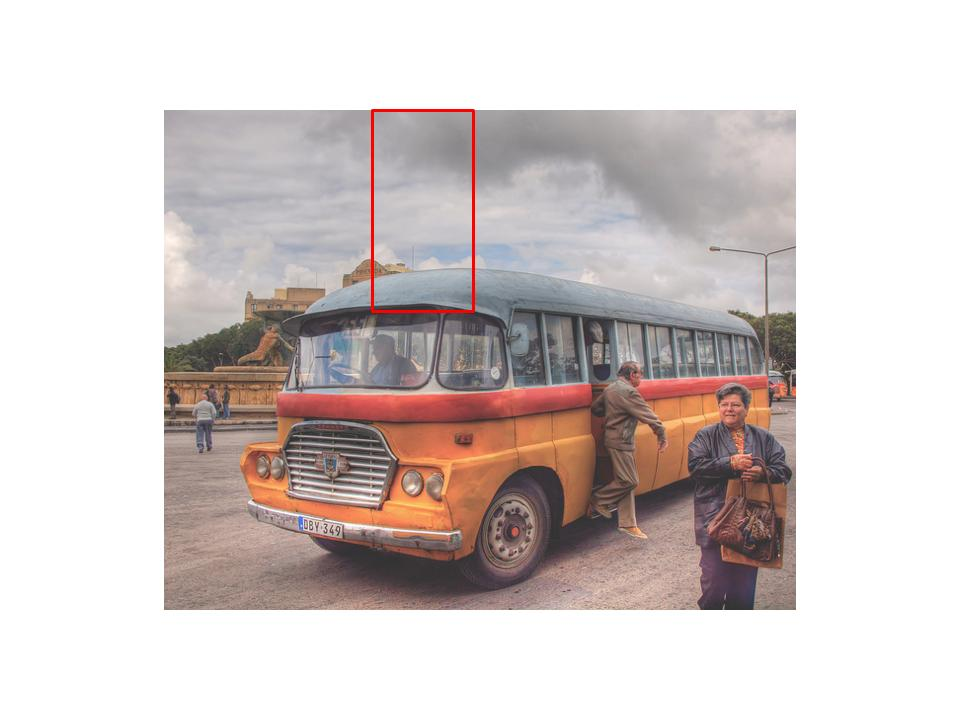
\includegraphics[width=\linewidth]{sliding_window_c.jpg}
    \caption{}
  \end{subfigure}
  \hspace*{\fill} % separation between the subfigures
  \begin{subfigure}{0.48\textwidth}
    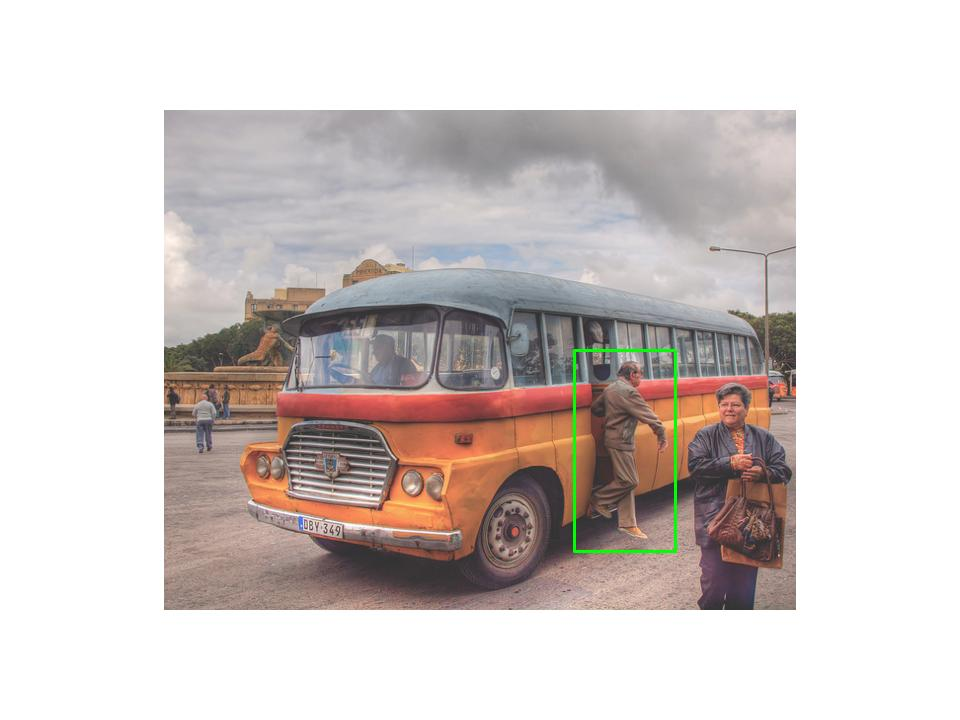
\includegraphics[width=\linewidth]{sliding_window_d.jpg}
    \caption{}
  \end{subfigure}
  \caption{Consider the problem of detecting people in an image. (a) - (c) sliding window across image and at each position classifying window as not containing a person. (b) window over person and classifying window as containing a person. Image source: Flickr user neilalderney123}
  \label{fig:sliding_window}
\end{figure}

\subsection{Feature Extraction and Object Representation}
Dalal and Triggs \cite{hog_human_detection} showed the effectiveness of using Histograms of Oriented Gradient (HOG) descriptors for human detection. Although their feature extraction methods were focused on human detection, they can be applied for detecting various objects. 

Recall HOG descriptors from lecture 8. An image window is divided into blocks; the magnitude of the gradients of the pixels in each block are accumulated into bins according to the direction of the gradients. These local histograms of the blocks are then normalized and concatenated to produce a feature representation of the image window.

\begin{figure}[H]
	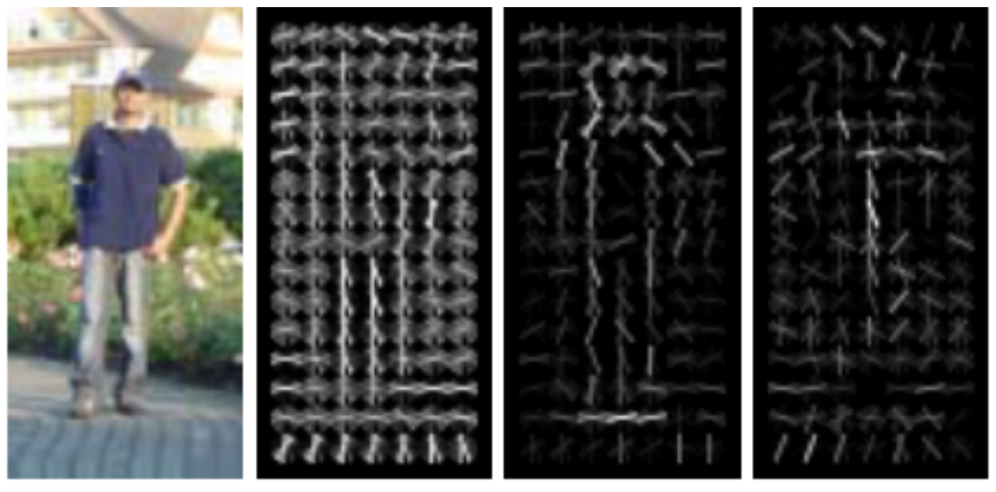
\includegraphics[width=\linewidth, scale=0.3]{person_template.png}
	\caption{An image of a person along with its respective HOG descriptor. Note that the last two images are the HOG descriptor weighted by the positive and negative weights of the classifier using them. The outline of the person is very visible in the weighted descriptors. Image source: Dalal and Triggs \cite{hog_human_detection}}
    \label{fig:hog_descriptor}
\end{figure}

Figure \ref{fig:hog_descriptor} shows an example of transforming an image into a HOG feature space. Producing a prototypical representation of an object would then involve considering many image windows labeled with containing that object. One approach to creating this representation would be to train a classifier on the HOG descriptors of these many labeled image windows and then proceed to use the trained classifier to classify the windows in images of interest. In their aim to improve human detection, for example, Dalal and Triggs \cite{hog_human_detection} train a linear Support Vector Machine on the HOG descriptors of image windows containing people.

A more simple approach, and the approach that will be assumed below, is that of averaging the window images containing an object of interest and then extracting the HOG descriptor of that average image to create a template for the object (Figure \ref{fig:face_template}).

\begin{figure}[h]
	\center
	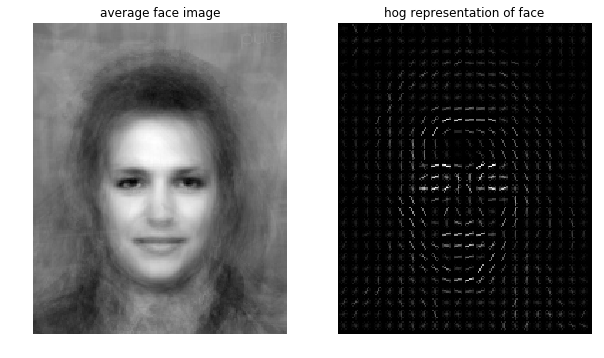
\includegraphics[scale=0.5]{average_face_template.png}
	\caption{The average face image above is created by averaging 31 aligned face images of the same size. The HOG descriptor of this average face image can then be used as a template for detecting faces in images.}
    \label{fig:face_template}
\end{figure}


\subsection{Classifying Windows}
Now that we have a method for extracting useful features from an image window and for constructing object templates, we can proceed to detecting objects in images. The idea is to compare each window with the object template and search for matches. That is, the object template itself acts as a filter that slides across the image. At each position, the HOG descriptor of the window being compared is extracted and a similarity score between the two HOG descriptors is computed. If the similarity score at some location is above a predefined detection threshold, then an object can be said to have been detected in the window at that location.

The similarity score can be as simple as the dot product of the window HOG descriptor and the template HOG descriptor. This is the scoring method that is assumed in following sections.

As effective as the method seems so far, it's success is very limited by the size of the sliding template window. For example, consider the case where objects are larger than the template being used to detect them (Figure \ref{fig:small_sliding_window}).

\begin{figure}[h]
  \begin{subfigure}{0.48\textwidth}
    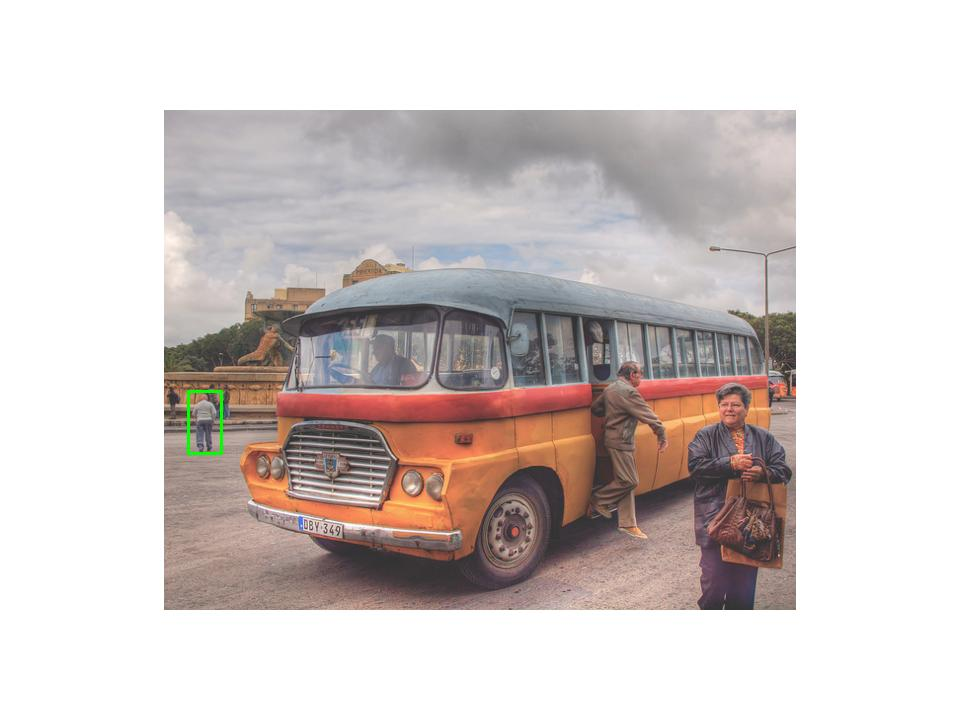
\includegraphics[width=\linewidth]{small_sliding_window_a.jpg}
    \caption{}
  \end{subfigure}
  \hspace*{\fill} % separation between the subfigures
  \begin{subfigure}{0.48\textwidth}
    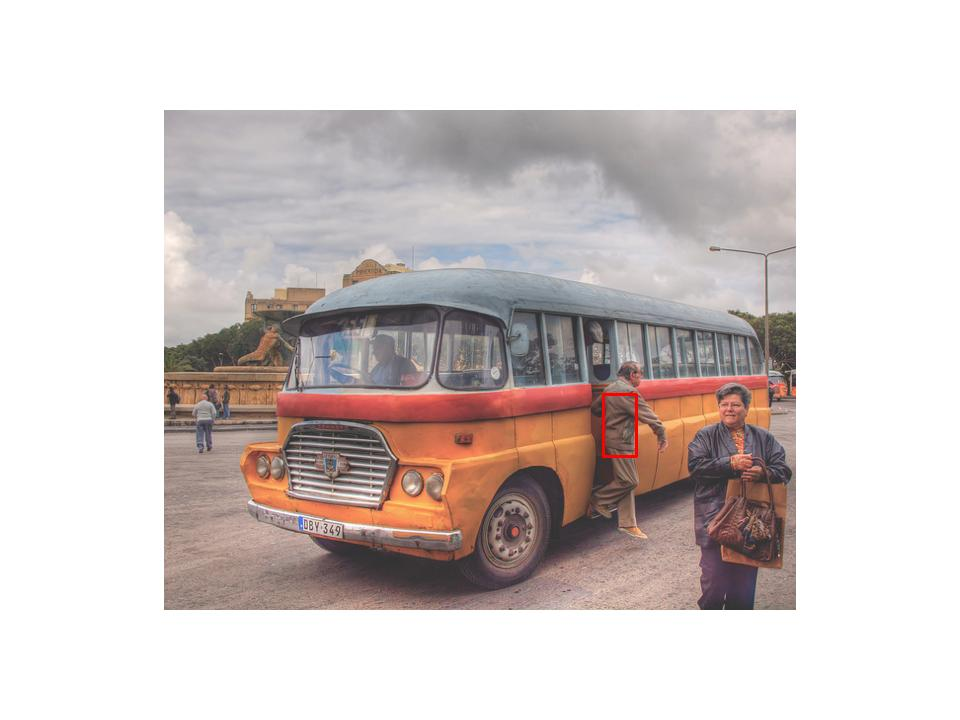
\includegraphics[width=\linewidth]{small_sliding_window_b.jpg}
    \caption{}
  \end{subfigure}
  \caption{Consider, again, the problem of detecting people, except this time our sliding window is much smaller. (a) The template and sliding window are still large enough to detect the smaller, distant person. (b) The person in the foreground is a lot bigger than our window size and is not being detected.}
  \label{fig:small_sliding_window}
\end{figure}

\subsection{Multi Scale Sliding Window}
To account for variations in size of the objects being detected, multiple scalings of the the image are considered. A feature pyramid (Figure \ref{fig:feature_pyramid}) of different image resizings is created. The sliding window technique is then applied as usual over all the the pyramid levels. The window that produces the highest similarity score out of the resizings is used as the location of the detected object.

\begin{figure}[h]
	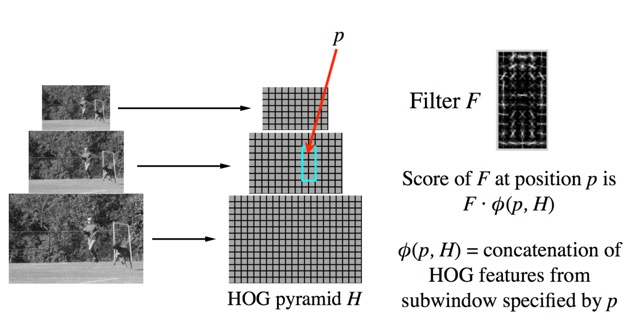
\includegraphics[width=\linewidth]{feature_pyramid.jpg}
	\caption{Using a feature pyramid of different image resizings allows the object template to match with objects that might have originally been bigger or much smaller than the the template. Image source: Lecture 15, Slide 40}.
    \label{fig:feature_pyramid}
\end{figure}

\section{The Deformable Parts Model (DPM)}
The simple sliding window detector is not robust to small changes in shape
(such as a face where the eyebrows are raised or the eyes are further apart, or cars
where the wheel's may be farther apart or the car may be longer) so we
want a new detection model that can handle these situations. Recall the
bag of words approach, in which we represent a paragraph as a set of words, or
an image as a set of image parts. We can apply a similar idea here and detect an
object by its parts instead of detecting the whole singular object. 
Even if the shape is
slightly altered, all of the parts will be present and in approximately the correct
position with some minor variance.\\

\subsection{Early Deformation Model for Face Detection}

In 1973, Fischler and Elschlager developed a deformable parts model for facial 
recognition \cite{DPM}: the parts of the face (such as eyes, nose, and mouth) are detected 
individually, and there are spring-like connections between each part that allows
each part to move slightly, relative to the other parts, but still largely conform
to the typical configuration of a face. This allows a face to be detected even if
the eyes are farther apart or a change in orientation pushes some parts closer 
together, since each part has some flexibility in its relative location in the face.
See Figure \ref{fig:deformable_face} for illustration\\

\begin{figure}[h]
	\center
	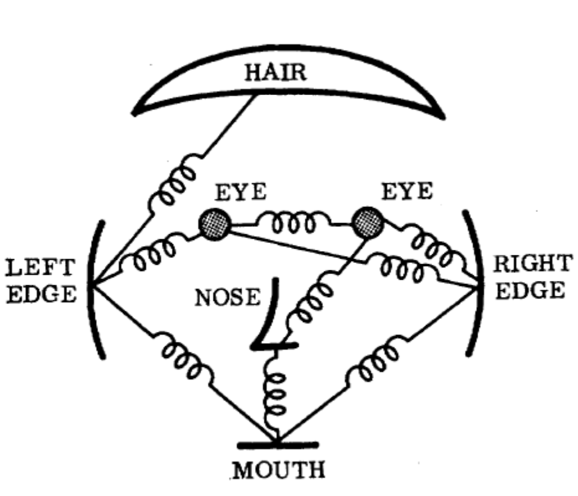
\includegraphics[width=0.4\textwidth]{deformable_model.png}
    \caption{An illustration of Fischler and Elschlager's deformable face model\cite{DPM}}.
    \label{fig:deformable_face}
\end{figure}

More formally, the springs indicate that there is a desired relative position
between two parts, and just like a spring stretches or compresses, we allow some deviations from that desired position, but apply an increasing penalty for larger
deviations, much like a string pulls back harder and harder as it is stretched further.

\subsection{More General Deformable Parts Models}

The deformable model depicted in Figure \ref{fig:deformable_face} is one specific 
deformable model for face detection, where Fischler and
Elschlager chose springs between parts that worked well with their methods for face 
detection. For a more
general deformable parts model, one popular approach is the star-shaped model, in
which we have some detector as the root and we have springs between every other
part and the root (see Figure \ref{fig:star_model}a for illustration)

\begin{figure}[h]
	\centering
	\begin{subfigure}{0.48\textwidth}
        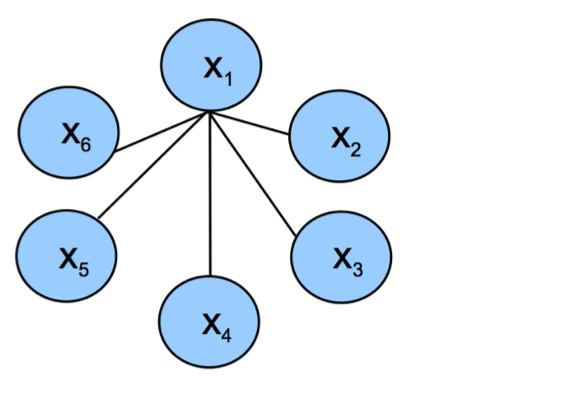
\includegraphics[width=0.8\textwidth]{star.png}
        \caption{}
    \end{subfigure}
    \hspace*{\fill} % separation between the subfigures
    \begin{subfigure}{0.48\textwidth}
        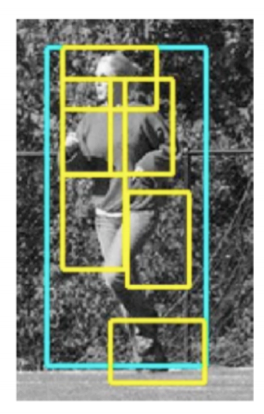
\includegraphics[width=0.48\textwidth]{person_star.png}
        \caption{}
    \end{subfigure}
    \caption{On the left is a visualization of the star model, with x1 as the root,
    and on the right is an example of person detection with a star model for 
    deformations}
    \label{fig:star_model}
\end{figure}

In face-detection, for example, we could have a detector for
the entire body as the root and thus define the location of all body parts relative
to the location of entire body. This is shown in Figure \ref{fig:star_model}b,
where the cyan box is the location of the bounding box from global person detection (which we use as the 
root) and the yellow boxes are the bounding boxes resulting from the detection of each part.\\

This means that
the head should be near the top-center of the global location of the person, the
feet should be near the bottom, the right arm should be near the left of image 
(if detector is for a front facing person), etc. In this class we will assume that we 
already know which parts to use (such as head,
arms, and legs if we are detecting people), but it is possible to learn the parts for
optimal object detection through machine learning\\

\subsection{Examples of Deformable Parts Models}
It is typical to use a global detector for the desired object (such as a person or
a bike) as the root, and to use smaller and more detailed filters to detect each
part. As a simple example, see Figure \ref{fig:deformable_head_filter}\\

\begin{figure}[h]
	\center
	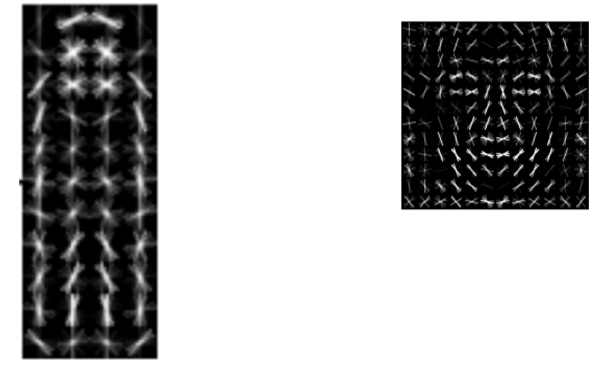
\includegraphics[width=0.5\textwidth]{deformable_head_filter.png}
    \caption{A global HOG filter for a person and a more detailed HOG filter for the 
    head}
    \label{fig:deformable_head_filter}
\end{figure}



It is also common to use a multi-component model for multiple orientations
of an object, in which we have a global filter and multiple parts filters for each
orientation. A deformable model will protect against the changing positions of parts
due to mild rotation, but for more significant rotations such as 90 degrees, all of
the parts looks different and require different detectors for each rotation. 
As an example, in figure
\ref{fig:car_model}, each row corresponds to an orientation. Also, the left column is a
global car detector for a particular orientation, the middle column contains all of the 
finer detailed parts filters for that orientation, and the right column shows the deformation penalties for
each part in that orientation (where darker grey in the center is smaller penalties and white further from
the center is larger penalties).\\

\begin{figure}[H]
	\center
	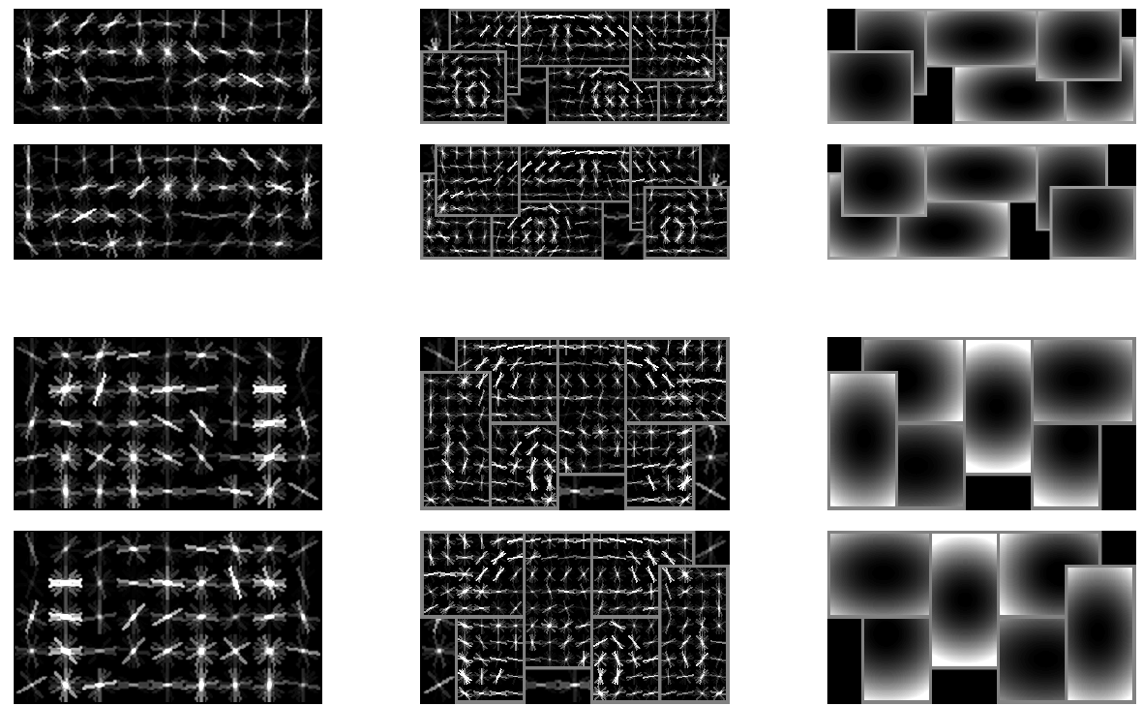
\includegraphics[width=0.9\textwidth]{car_model.png}
    \caption{Deformable Parts model of a car with multiple orientations}
    \label{fig:car_model}
\end{figure}

As another example, consider 2 orientations for bike detection. A bicycle looks very
different from the front and from the side so we want multiple detectors. Here we can
see the parts identified in the original image alongside the deformable model

\begin{figure}[h]
	\center
	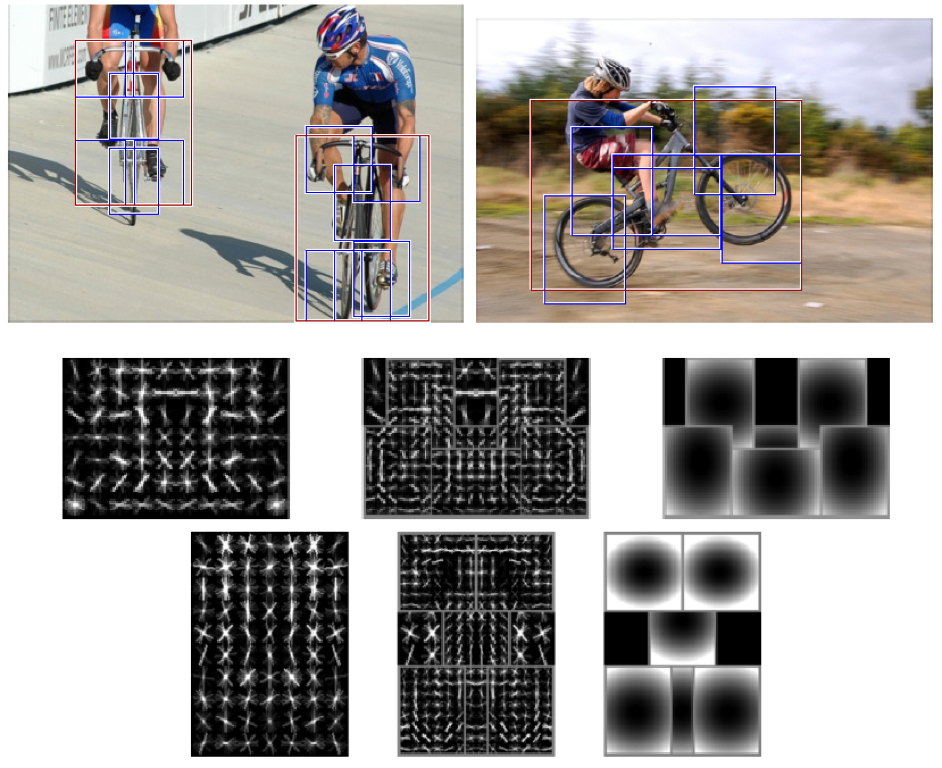
\includegraphics[width=0.9\textwidth]{deformable_bike_model.png}
    \caption{Deformable Parts model of a bike with original image shown}
    \label{fig:deformable_bike_model}
\end{figure}



\subsection{Calculating Score for Deformable Parts Models}

To implement a deformable parts model we need a formal way to calculate score. To do
this we will calculate a global score from the global object detector, and then
calculate a score for each part, determined by it's deformation penalty. The final
score is the global score minus all of the deformation penalties, such that an object
that is detected strongly but has many of the parts very far from where they should be will be highly penalized.\\

To express this more formally we will first define some variables: The entire model with n parts is
encompassed by an (n+2) tuple: $$(F_0, P_1, P_2, ... P_n, b)$$
where $F_0$ is the root filter, $P_1$ is the model for the first part, and $b$ is a 
bias term. Breaking it down further, each part's model $P_i$ is defined by a tuple
$$(F_i, v_i, d_i)$$
where $F_i$ is the filter for the i-th part, $v_i$ is the "anchor" position for part
i relative to the root position, and $d_i$ defines the deformation cost for each
possible placement of the part relative to the anchor position.\\


We can calculate the location of the global filter and each part filter
with a HOG pyramid (see Figure \ref{fig:deformable_score1}). We run the global HOG
filter
and each part's HOG filter over the image at multiple scales so that the model is 
robust
to changes in scale. The location of each filter is the location where we see the
strongest response. Since we are taking the location of responses across multiple
scales we have to take care that our description of the location of each part is
scale-invariant (one way this can be done is by scaling the maximum response map for 
each part up to the original image size and then taking scale-invariant location).\\

\begin{figure}[h]
	\center
	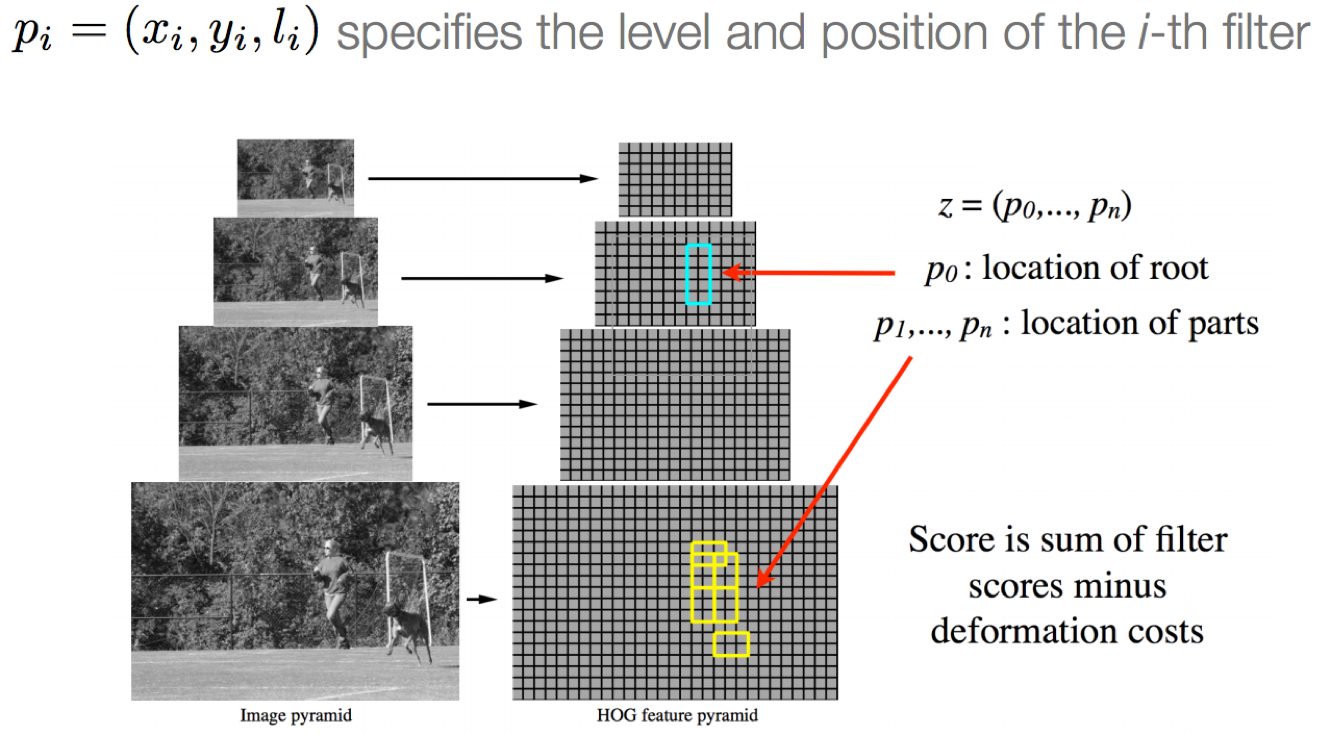
\includegraphics[width=0.9\textwidth]{deformable_score1.png}
    \caption{Illustration of HOG pyramid for deformable parts detector}
    \label{fig:deformable_score1}
\end{figure}

We calculate the detection score as 
$$\prod_{i=0}^{n}F_i \cdot \phi(p_i,H) - \sum_{i=1}^{n}d_i(dx_i,dy_i,dx_i^2, dy_i^2)$$

Taken as a whole, this means that we are finding detection score of the global root and 
all the parts and subtracting all of the deformation penalties.\\

The left term represents the product of the
scores for the global filter and each
part filter (note that this is identical to the simpler Dalal and Triggs \cite{hog_human_detection} or sliding
window method explained previously).
Recall that the score for each filter is
the inner product of the filter (as a vector) and $\phi(p_i,H)$ (defined as
the HOG feature vector of a window defined by position $p_i$ of the filter). Note
that the windows can be visualized in the HOG pyramid in Figure 
\ref{fig:deformable_score1}: the window for the root is the cyan bounding box, and the window
for each of the parts is the yellow bounding box corresponding to that part. We are taking
the HOG feature vector of the portion of the image enclosed in these bounding boxes and seeing how well it matches with the HOG features of the template for that part.\\

Returning to the score formula, the right term represents the sum of the 
deformation penalties for each part.
We have $d_i$ representing the weights of each penalty for part i, corresponding to quantities
$dx_i$ (the distance in x direction from the anchor point where the part should be), 
$dy_i$ (the distance in y direction from the anchor point where the part should be), as 
well as $dx_i^2$ and $dy_i^2$. As an example, if $d_i = (0, 0, 1, 0)$, then the 
deformation penalty for part i is the square of the distance in the x direction of
that part from the anchor point. All other measures of distance are ignored.\\

\section{The DPM Detection Pipeline}

\begin{figure}[ht]
	\center
	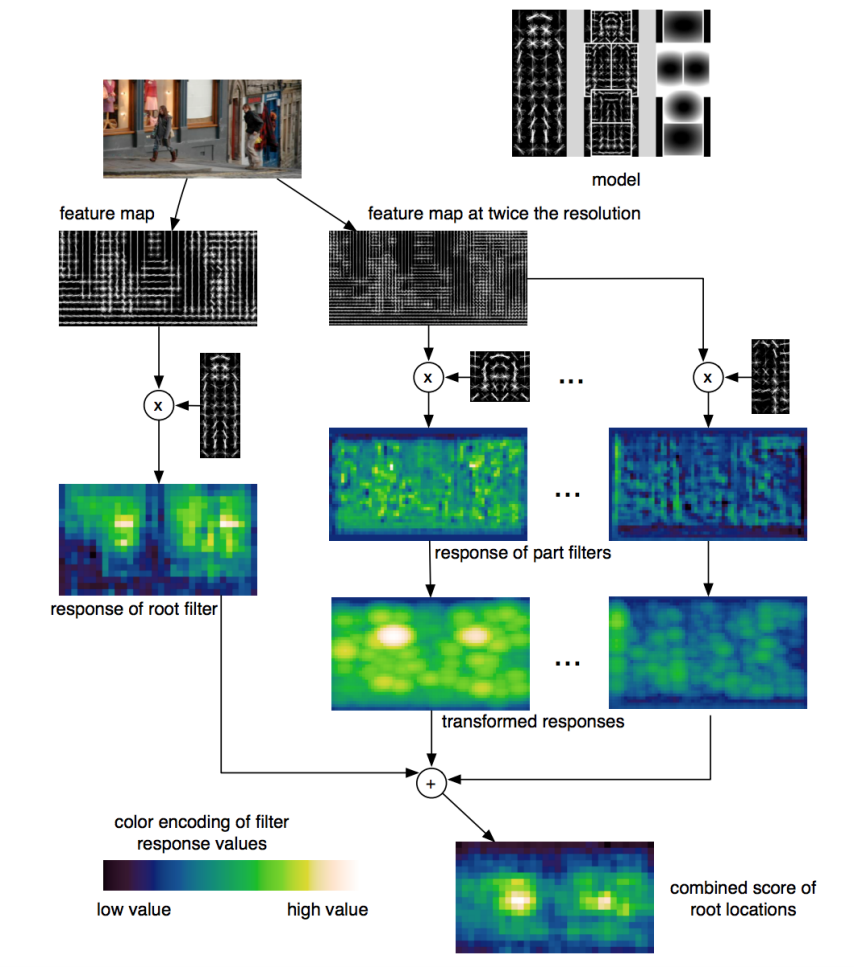
\includegraphics[scale=0.6]{pipeline.png}
    \caption{Illustration of full DPM Pipeline}
    \label{fig:pipeline1}
\end{figure}


The Deformable Parts Model detection pipeline has several stages. We must first use the global filter to detect an object. Then, the parts filters are used to calculate the overall score of that detection.
\begin{enumerate}
\item Generate copies of the original image at different resolutions (so that the fixed window size can capture objects at varied scales); store the HOGs for these different resolutions, as that is what the filters will be applied to.



\begin{figure}[H]
	\center
	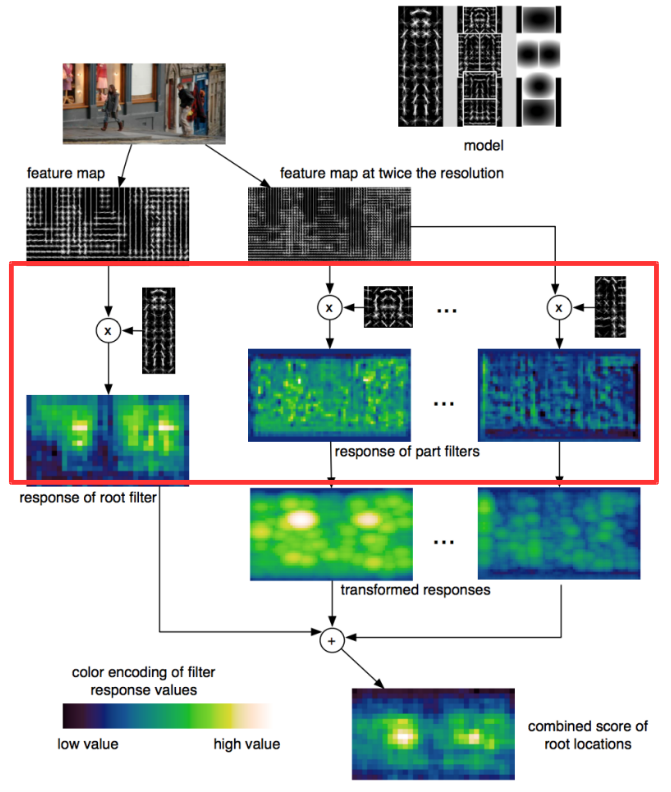
\includegraphics[scale=0.2]{pipeline2a.png}
    \caption{Step 2 of the detection pipeline}
    \label{fig:pipeline2a}
\end{figure}
\item Apply the global filter to these images. Upon a detection by the global filter, apply the parts filters. This step represents the section of the pipeline depicted in Fig. \ref{fig:pipeline2a}, and contributes the term:

$$\prod_{i=0}^{n}F_i \cdot \phi(p_i,H)$$



\item Having applied the parts filter, we now calculate the spatial costs (i.e., a measure of the deformation of the parts with regards to the global):

$$ \sum_{i=1}^{n}d_i(dx_i,dy_i,dx_i^2, dy_i^2) $$

\begin{figure}[h!]
	\center
	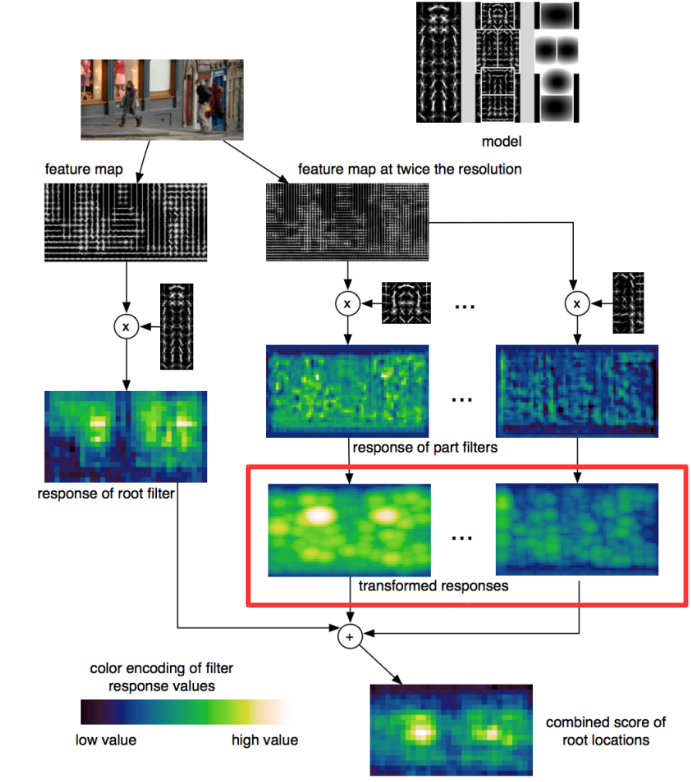
\includegraphics[scale=0.2]{pipeline2b.png}
    \caption{Step 3 of the detection pipeline}
    \label{fig:pipeline2b}
\end{figure}


\item For every detection, we now sum these components to calculate the \textit{detection score}:

$$ F_0 + \prod_{i=1}^{n}F_i \cdot \phi(p_i,H) - \sum_{i=1}^{n}d_i(dx_i,dy_i,dx_i^2, dy_i^2)$$

\item These scores then represent the strength of the detection of the given object at each coordinate of the image; hence, we can plot the response scores throughout the image:

\begin{figure}[h!]
	\center
	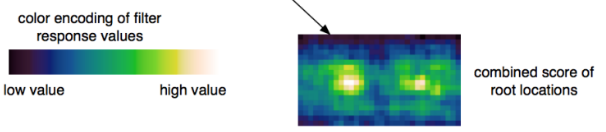
\includegraphics[scale=0.5]{pipelinescoreplot.png}
    \caption{Response scores}
    \label{fig:pipelinescoreplot}
\end{figure}

\end{enumerate}

\section{DPM Detection Results}

The Deformable Parts Model makes some key assumptions: an object is defined by a relationship between a global representation (e.g., a car) and representations of parts (e.g. wheels, or a bumper); that the strength of this detection increases with the decrease in deformation between the root and the parts; and that if a high response score is achieved, that object is indeed present (regardless of the potential presence of different categories of objects). Hence, DPM is vulnerable to error in situations where these assumptions are violated:

\begin{figure}[h!]
	\center
	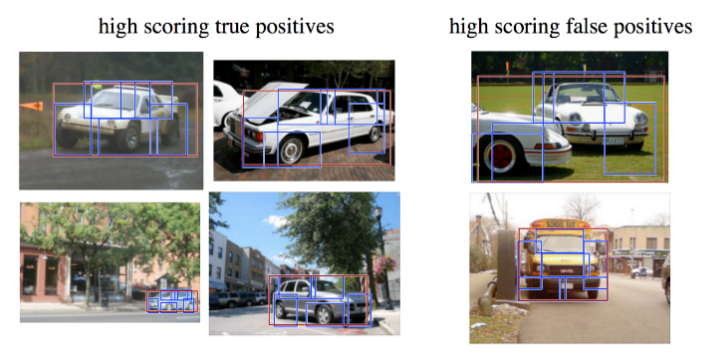
\includegraphics[scale=0.6]{results-tpfp.png}
    \caption{Typical errors for the DPM model}
    \label{fig:results-tpfp}
\end{figure}



Note how in the top image on the right, DPM has successfully found sections matching the parts filters: wheels and a windshield. DPM has also successfully found one true positive for the global filter (the car in the background). However, DPM assumes that these parts are related to each other because they are spatially close (i.e., they fit the deformation model), and that they correspond to the car identified as the global filter -- when in reality, there is not one but two cars in the image providing the parts.

Similarly, with the bottom image, DPM indeed detects an object very close to a car. However, since it does not take into account that the object is even closer to being a bus than a car, and does not take into account features explicitly \textit{not} present in a car (e.g., the raised roof spelling "School bus"), DPM results in a wrong detection.
\section{DPM Summary}
  \textbf{Approach}
  \begin{itemize}
  \item Manually selected set of parts: a specific detector is trained for each part
  \item Spatial model is trained on the \textit{part} activations
  \item Joint likelihood is evaluated for these activations
  \end{itemize}

  \textbf{Advantages}
  \begin{itemize}
  \item Parts have an intuitive meaning
  \item Standard detection approaches can be used for each part
  \item Works well for specific categories
  \end{itemize}

  \textbf{Disadvantages}
  \begin{itemize}
  \item Parts need to be selected manually
  \item Semantically motivated parts sometimes don’t have a simple appearance distribution 
  \item No guarantee that some important part hasn’t been missed
  \item When switching to another category, the model has to be rebuilt from scratch
  \end{itemize}

  Notably, the Deformable Parts Model was state-of-the-art 3-4 years ago, but has since fallen out of favor. Its "fully-connected" extension, pictured below, is particularly no longer used in practice:

  \begin{figure}[h!]
      \center
      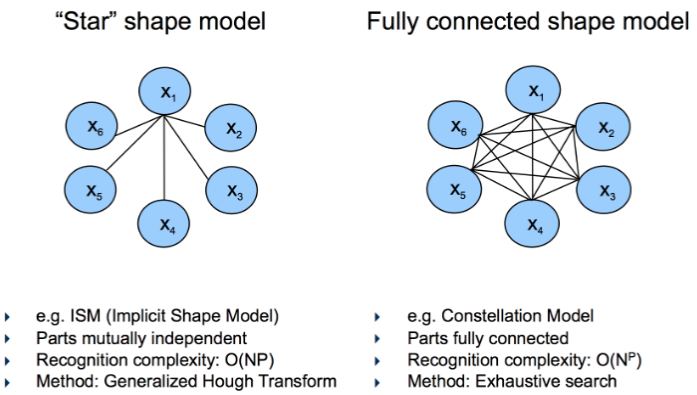
\includegraphics[scale=0.55]{fullyconnected.png}
      \caption{DPM extension: fully-connected shape model}
      \label{fig:fullyconnected}
  \end{figure}

\newpage
% References
\small
\bibliographystyle{plain}
\bibliography{bibliography}
\end{document}
